\section{Past Work}

Asure’s primary focus within the social security field is on pension insurance. As part of the ongoing research, we have ported the specific aspects of the German pension system to Ethereum blockchain. Based on both, our hands-on experience and our expertise from years of working in the insurance field, we developed the theoretical backbone of how a decentralized pension system is supposed to function as well as the proof-of-concept implementation of such a system. 

\subsection{Research on the blockchain technology and automation}

Asure’s CTO, Fabian Raetz, did a research project at the University of Applied Science and Art Dortmund in 2013 where he analyzed the emerging blockchain technologies and its possible applications. \cite{fraetz}
\newline

In 2014 a small team led by Paul Mizel and Fabian Raetz developed their own blockchain based currency as a proof of concept and tested different kinds of blockchain issues and economic systems (NRJ Coin). \cite{nrjcoin}
\newline

Paul Mizel has built a team in Kiev late 2015 for AI-based innovation projects  “Insure Chat”, “Insure Assistant” and “Insure Advisor”. The applications that were built as a result were fully automated chatbots for support, claim management, and other tasks with a unique learning mechanism and connection to social platforms like Facebook, Telegram, Skype, and others.\newline
Tech stack: IBM Watson, Microsoft Bot Framework, MS Luis, .NET.
\newline
Algorithms used: Text mining, regression analysis, SVMs, neural networks.

\subsection{German Pension System}
In order to demonstrate the potential of blockchain-based social security, Asure created a prototype based on the model of the German statutory pay-as-you-go pension system.
\newline\newline

The Asure dApp will become the reference implementation for dApps using the Asure blockchain and platform.
\newline\newline
It will feature
\begin{itemize}
\item a technical feasibility study of the german statutory pension system implemented on the Ethereum blockchain and the Asure protocol / platform.
\item a complete wallet implementation.
\item an overview and management of your insurance policies.
\item an insurance store to find and buy insurance policies.
\end{itemize}

Please try out the Asure dApp which runs currently on the Ethereum Rinkiby testnet: 
https://dapp.asure.io

\subsection{Decentralized Pension System}

To demonstrate that blockchain can solve problems globally, Asure also developed a prototype of a global pension system which is fully decentralized and hence lies neither in the hands of governments nor of any insurance company.

This is an alpha-phase experiment designed to show how social security systems can be improved in the future with the help of blockchain technology.

The idea is to implement a pay-as-you-go pension system on Ethereum blockchain. Members pay their contributions in ETH and receive ERC20 tokens in return. No contributions are invested in the capital market and therefore no interest is earned. Instead, the paid-in ETHs are used directly for the payment of outstanding pension claims. How much pension is going to be paid out depends on how many pension tokens a pensioner has, i.e. how many contributions he paid into the system.

As a rule, pay-as-you-go systems only work because states introduce mandatory social security systems and, thus can guarantee a stable number of members and contribution payments. In a decentralized pension system nobody can be forced to become a member. Asure's membership creates several incentives that are intended to lead to mass acceptance.

In the decentralized pension system as well as in a classic one, whoever makes a higher contribution gets a higher pension. Pay-ins longevity plays a role as well. The longer one makes regular pay-ins the longer the pension is going to be paid out.

\begin{figure}[H]
    \centering
    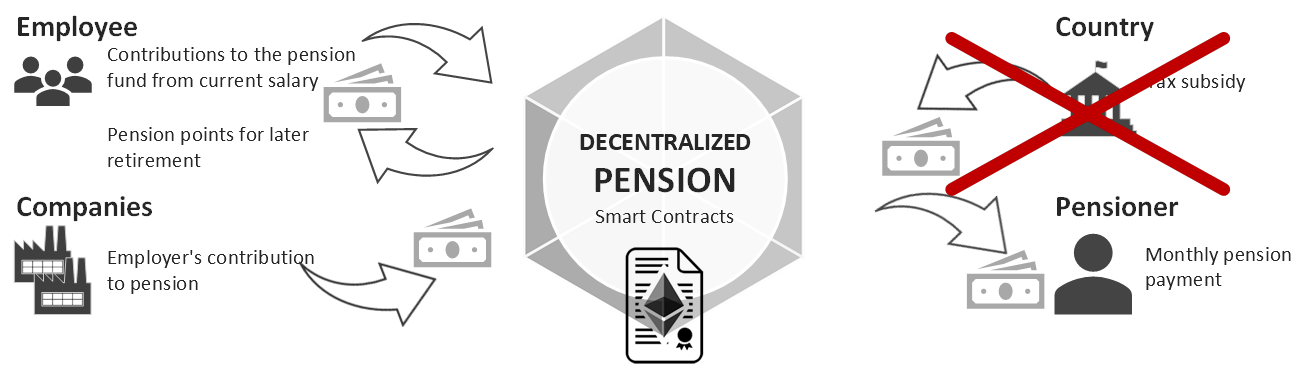
\includegraphics[width=5.0in]{img/pension.png}
    \caption{PAYG Model}
    \label{fig:payg}
\end{figure}

The Asure decentralized pension dApp runs currently on the Ethereum Rinkeby testnet. It was developed during ETHBerlin hackathon and can be accessed via the following link: 
\url{https://ethberlin.asure.io}

Pension is a bet that the value I pay in is at least as great, if not greater, as the payout. The decentralized pension is based on the German pension system and has implemented a “generation contract”. The young generation pays the older generation according to their possibilities and in return, the pension entitlements are tokenized, In the form of pension entitlement tokens (PET).
\newline\newline

\subsubsection*{Incentive models were developed within the project}
The system excludes the administration of age, thereby avoiding fraud and evidence. The time is divided into periods where a period is a month. Within each period deposits can be made. For each period a target price is fixed, which can shift if the median of the deposits of the previous period has a big difference to the target price. 

If the maximum number of periods has been paid in, the maximum number of pension payments is also possible. Let's assume that the maximum number of periods is 480 equal 40 years. For monthly payments of 40 years, there is a claim to 40 years pension. If someone has only used the system for 2 years, the application is for 1 month only. The incentive to use the system to the maximum rewards the participants with more pension entitlement period.

\begin{eqnarray}
	entitlementMonths = \frac{payedMonths^2}{12 \cdot 40 years}
\end{eqnarray}

\begin{figure}[H]
    \centering
    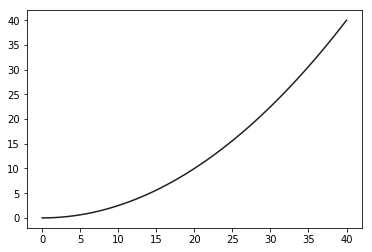
\includegraphics[width=3.0in]{img/pension_years.png}
    \caption{Decentralized pension payed vs. recive years}
    \label{fig:pension_years}
\end{figure}

Since everyone can pay in different amounts in the system, the maximum payer is granted a maximum of double pension entitlement. All those who pay in more than the target price of the period will receive more PET up to a maximum of 2 per period. Maximum achievable 960 PET, this allows a later claim to twice as much in redistribution as someone who activates 480 PET.

\begin{eqnarray}
	DPT = \begin{cases} 1 + \frac{amount-amount_{max}}
	{targetPrice - amount_{max}} 
	* DTP_{bonus} & amount \geq targetPrice\\
	\frac{amount - amount_{min}}
	{targetPrice - amount_{min}} 
	* DTP_{bonus} & otherwise\end{cases}
\end{eqnarray}

\begin{eqnarray}
targetPrice - amount_{max} \neq 0 \quad and \quad targetPrice - amount_{min} \neq 0
\end{eqnarray}

As a further incentive for the early adopters, a bonus was provided in the system which has a multiplicator of 1.5 and with the time logarithmically approaching 1.0 is planned to approach annually.

\begin{eqnarray}
	DTP_{bonus} = f(year) = 1.5-0.12 * log(year)
\end{eqnarray}

\begin{figure}[H]
    \centering
    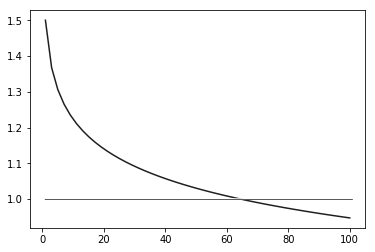
\includegraphics[width=3.0in]{img/pension_bonus.png}
    \caption{Decentralized pension bonus by year}
    \label{fig:pension_bonus}
\end{figure}

If everyone leaves the system, the last participants are rewarded more, thus we guarantee that the system remains lucrative, with zero participants in the system the system is set to its initial state again.

By the limitation on maximally 2 PET or with the factor 1.5 initially 3 PET per period in the first years a utilization possibility results with several accounts into the system to pay in which the system prevents that the PETs are not transferable. 

With the help of these incentives and transparent design and DAO approach, this will start as a social experiment after necessary simulations and parameter adjustments on Ethereum mainnet.

\subsubsection*{Benefits}
Independent Crypto Pension has many advantages, the intergenerational contract allows the inflation security. It is autonomous and decentralized according to the idea of the DAO. There is no intermediary.  The privacy is secured because no personal data is necessary to participate in the system.  It is completely transparent as all transactions are on the blockchain and it is also open source.

\subsubsection*{Read more}
We summarized our ideas on how a redistribution based peer-to-peer pension system might look and share our results with the broader community.
\newline
Depot Paper: \url{https://www.asure.network/asure.depot.en.pdf}

